% =============================================================
% DS4H Tutorat Report - M1 Informatique
% Compile on Overleaf with pdfLaTeX. Self-contained (TikZ/pgfplots).
% =============================================================
\documentclass[11pt,a4paper]{article}

\usepackage[T1]{fontenc}
\usepackage[utf8]{inputenc}
\usepackage[english]{babel}
\usepackage{lmodern}
\usepackage[a4paper,margin=2.4cm]{geometry}
\usepackage{microtype}

\usepackage{amsmath,amssymb,amsfonts}
\usepackage{graphicx}
\usepackage{booktabs}
\usepackage{array}
\usepackage{caption}
\usepackage{subcaption}
\usepackage{float}
\usepackage{xcolor}
\usepackage{listings}
\usepackage{enumitem}
\usepackage{titlesec}
\usepackage{fancyhdr}

\usepackage{tikz}
\usetikzlibrary{positioning,arrows.meta,shapes.geometric,fit,backgrounds,calc,chains}
\usepackage{pgfplots}
\pgfplotsset{compat=1.18}

\usepackage[hidelinks]{hyperref}
\usepackage{cleveref}

\titleformat{\section}{\Large\bfseries}{\thesection}{0.6em}{}
\titleformat{\subsection}{\large\bfseries}{\thesubsection}{0.6em}{}
\titleformat{\subsubsection}{\normalsize\bfseries}{\thesubsubsection}{0.6em}{}

\pagestyle{fancy}
\fancyhf{}
\fancyhead[L]{\small Tutorship -- M1 Informatique DS4H}
\fancyhead[R]{\small \thepage}
\renewcommand{\headrulewidth}{0.4pt}

\lstset{
  basicstyle=\ttfamily\small,
  frame=single,
  framerule=0.4pt,
  framesep=4pt,
  xleftmargin=8pt,
  xrightmargin=4pt,
  breaklines=true,
  showstringspaces=false,
}

\newcommand{\rqone}{\textbf{RQ1}}
\newcommand{\rqtwo}{\textbf{RQ2}}
\newcommand{\rqthree}{\textbf{RQ3}}

% =============================================================
\begin{document}

\begin{titlepage}
\centering
    \centering
    \thispagestyle{empty}
    
    \vspace*{1cm}
    
    % Logo Section
    \includegraphics[width=0.7\textwidth]{EUR-DS4H_annuaire.jpg} 
    
\vspace{4.0cm}
\rule{\linewidth}{0.5pt}\par
\vspace{0.4cm}
{\huge\bfseries Automatic solving of combinatorial problems and their explanations using LLMs and constraint programming \par}
\vspace{0.2cm}
\vspace{0.8cm}
\rule{\linewidth}{0.5pt}\par
\vspace{2.0cm}

\begin{tabular}{ll}
\textbf{Student} & Oussama Belhout \\
\textbf{Student ID} & 22410451 \\
\textbf{Programme} & M1 Informatique \\
\textbf{Supervisor} & Pr.Jean-Charles Régin \\
\textbf{Host laboratory} & I3S \\
\textbf{Recipients} &
Dr.Cinzia Di Giusto,\vspace{0.1cm} Dr.Anne-Laure Simonelli \\
\textbf{Project period} & Spring 2026 \\
\end{tabular}

\vfill
{\large Tutorship final report \par}
{\large Submission: 12 May 2026 \par}
\end{titlepage}

\section*{Abstract}
Many real-world tasks reduce to choosing values for a set of decision variables under a list of rules: routing delivery trucks, scheduling hospital staff, allocating compute jobs to GPUs. Specialised programs called solvers handle the search efficiently, but only when the problem is first written in their own formal input language. The present work studies whether a Large Language Model (LLM) can produce that formal input from a natural-language description.

Three design choices govern such a system: the prompting technique $\pi$, the LLM $m$, and the agentic design $\alpha$ (the number of LLM calls and how they are connected). Every configuration $c = (\pi, m, \alpha)$ was run on the same ten CSPLib problems with three LLMs. The agentic-design axis was then studied through the Progressive Delegation Ablation (PDA), a four-level ladder from a single all-in-one agent (L0) to a chain of four specialised agents (L3).

Under the conditions tested, mean success rate falls monotonically across the ladder: $100\%$ at L0, $93.3\%$ at L1, $80.0\%$ at L2, $66.7\%$ at L3, with the four hard problems driving the entire decline. Five mechanisms are proposed and unified under one principle, named here the \emph{verifier-redundancy tax}: when an exact deterministic checker is already available, adding LLM agents tends to compete with that checker rather than help it.
\vspace{0.4cm}
\hrule
\vspace{0.4cm}
\textbf{Keywords:} Constraint Satisfaction Problems; Large Language Models; multi-agent systems; neuro-symbolic systems; ablation study; Choco solver; CSPLib.

\newpage
\vspace{0.4cm}  
\hrule
\vspace{0.4cm}

\tableofcontents
\newpage

% =============================================================
\section{Introduction}\label{sec:intro}

\subsection{Why combinatorial problems matter}\label{sec:intro:why}
Many of the hardest problems in modern technology start with a short description and explode into something no human can solve by hand. Routing a fleet of delivery trucks across a city, scheduling staff in a hospital, assigning tasks to a team of robots, allocating compute jobs to a cluster of GPUs, and laying out the transistors of a microchip all share the same underlying mathematical structure: choose values for a set of decision variables under a list of rules.

The difficulty is not the description; the difficulty is the size of the choice space. A distribution of twenty employees over seven shifts admits more than $10^{20}$ different assignments. Listing them one by one is impossible, even on a fast computer. Special-purpose programs called \emph{solvers} can search such choice spaces without listing every candidate~\cite{R1}. They form the engine behind airline scheduling, factory planning, and chip design.

A solver, however, does not accept everyday language as input. It accepts only a \emph{formal model}: a precise description written in the solver's own input language. Writing the formal model is the real bottleneck. The task requires both mathematical training and detailed familiarity with the specific solver in use. Such expertise remains scarce. The motivation of the present work is to replace the human modeller by an automated component.

\subsection{Why language models are a candidate}\label{sec:intro:llm}
A Large Language Model (LLM) is a neural network trained on very large amounts of text. It accepts a problem stated in natural language, that is, the way a human would describe it, and produces text in response, including code. An LLM is therefore a plausible candidate to translate a natural-language problem statement into the formal model that a solver requires~\cite{R3}.

The role of the LLM in the system studied here is intentionally limited. The LLM produces the formal model. The actual search through the choice space is performed by the solver. The LLM never explores the space itself, because LLM outputs are \emph{probabilistic} and offer no guarantee of correctness. The solver, in contrast, is \emph{deterministic}, in the strict sense: identical input produces identical output on every run. The task dispatch between a probabilistic component (the LLM) and a deterministic component (the solver) is the defining feature of \emph{neuro-symbolic} systems~\cite{R7}, described in Section~\ref{sec:bg:neurosymbolic}.

\subsection{Three design choices}\label{sec:intro:axes}
Building such a system requires three design choices.

The first design choice is the \emph{prompting technique}, denoted $\pi$. A prompting technique is the template used to phrase the request given to the LLM. The template may contain instructions, worked examples, and conditions to respect on the expected output format.

The second design choice is the \emph{LLM} itself, denoted $m$. Different LLMs differ in size, in the data on which they were trained, and in their reliability when generating code.

The third design choice is the \emph{agentic design}, denoted $\alpha$. An \emph{agent}, in this report, is one LLM call configured to perform one specific task. An agentic design specifies how many agents the system contains and how the output of each agent is passed to the next.

A configuration of the system is denoted by the triple
\[
c = (\pi, m, \alpha) \in \mathcal{C} = \Pi \times M \times A,
\]
where $\Pi$, $M$, and $A$ are the sets of prompting techniques, LLMs, and agentic possible designs that are considered. The three design choices combine to form the final result. A stronger LLM can compensate for a weaker prompting technique. A deeper agentic design can amplify a small per-agent error rate. Varying only one of the three at a time would mix effects together; varying all three jointly and recording the outcome for every combination makes it possible to attribute each observed effect to the right design choice.

One further property makes the present study particularly attractive. The combinatorial solver under consideration is generic: the same solver handles 4-Queens, scheduling, Sudoku, and graph colouring without modification. Specialised algorithms exist for each of these problems, but every such algorithm only solves the one problem it was designed for. A successful natural-language interface to a generic solver therefore unlocks many problems at once, instead of one problem at a time.

\subsection{Research questions}\label{sec:intro:rq}
Three research questions guide the study.
\begin{itemize}[leftmargin=1.4em,topsep=2pt,itemsep=1pt]
  \item \rqone{}. How can LLMs be used to solve Constraint Satisfaction Problems?
  \item \rqtwo{}. Which configuration $c \in \mathcal{C}$ produces the highest success rate on the benchmark problems used here?
  \item \rqthree{}. Can the system correct its own errors without human intervention when a generated model fails to compile or to satisfy the problem?
\end{itemize}

\subsection{Contributions}\label{sec:intro:contrib}
This work makes four contributions.
\begin{enumerate}[leftmargin=1.4em,topsep=2pt,itemsep=1pt]
  \item An \emph{enumeration of all design combinations}: every triple $(\pi, m, \alpha)$ in the configuration space $\mathcal{C}$ was run on the same benchmark suite, with the same metrics recorded for each cell. The enumeration provides a direct, measured answer to \rqtwo{}.
  \item A focused study of the agentic-design axis, named the \emph{Progressive Delegation Ablation} (PDA). The word \emph{ablation} here means a controlled experiment in which one design choice (the number of agents) is varied while the other two are held fixed. The PDA compares four agentic designs $\alpha \in \{\mathrm{L0}, \mathrm{L1}, \mathrm{L2}, \mathrm{L3}\}$, in which L0 uses a single agent and L3 uses a chain of four specialised agents.
  \item A measured finding that contradicts a common assumption in the multi-agent-LLM literature~\cite{R5,R6}. On the benchmark suite tested here, the mean success rate decreases monotonically from $100\%$ at L0 to $66.7\%$ at L3 as the number of agents grows.
  \item An explanation of why the decline occurred, composed of five mechanisms (M1--M5) and unified under one named principle, the \emph{verifier-redundancy tax}.
\end{enumerate}

\subsection{Outline of the report}\label{sec:intro:outline}
Section~\ref{sec:bg} explains the background that the rest of the report relies on: what a CSP is, what an LLM is, and what a neuro-symbolic system is. Section~\ref{sec:method} describes how the experiment was set up. Section~\ref{sec:results} reports the numbers obtained. Section~\ref{sec:discussion} explains the numbers and proposes the verifier-redundancy tax. Section~\ref{sec:conclusion} concludes and lists future directions.

% =============================================================
\section{Background}\label{sec:bg}

\subsection{Constraint Satisfaction Problems}\label{sec:bg:csp}
A Constraint Satisfaction Problem (CSP) is described by three components: the \emph{decision variables}, the values each variable may take, and the rules the variables must obey. Formally, a CSP is a triple $\mathcal{P} = (V, D, C)$, where $V = \{v_1, \dots, v_n\}$ is the set of variables, $D = \{D_1, \dots, D_n\}$ assigns to each variable $v_i$ a finite set $D_i$ of admissible values, and $C$ is the set of constraints. A \emph{solution} of $\mathcal{P}$ is an assignment of one value from $D_i$ to each $v_i$ such that every constraint in $C$ is satisfied.

A small example is the 4-Queens problem, illustrated in Figure~\ref{fig:4queens} (an instance of CSPLib problem 054~\cite{R2}). Four queens must be placed on a $4 \times 4$ chessboard such that no two queens attack each other. Each variable $v_i$ stands for the column position of the queen in row $i$. Each domain $D_i$ is the set $\{1, 2, 3, 4\}$ of possible columns. The constraints state that no two queens share a column ($v_i \neq v_j$ for $i \neq j$) and that no two queens share a diagonal ($|v_i - v_j| \neq |i - j|$). The placement $(v_1, v_2, v_3, v_4) = (2, 4, 1, 3)$ satisfies every constraint.

\begin{figure}[H]
\centering
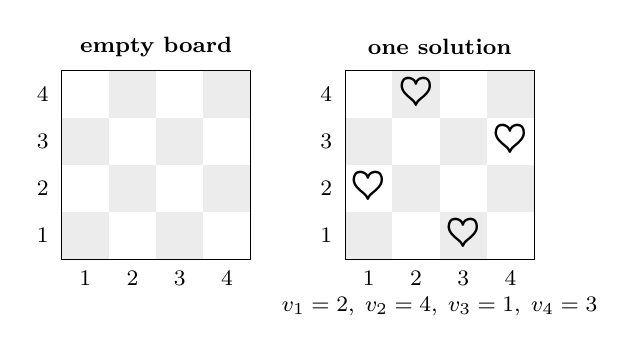
\begin{tikzpicture}[scale=0.6, every node/.style={font=\footnotesize}]
% Empty board on the left
\foreach \x in {0,1,2,3} {
  \foreach \y in {0,1,2,3} {
    \pgfmathparse{mod(\x+\y,2)==0 ? "gray!15" : "white"}
    \edef\cellcolor{\pgfmathresult}
    \fill[\cellcolor] (\x,\y) rectangle ++(1,1);
  }
}
\draw (0,0) rectangle (4,4);
\foreach \i in {1,2,3,4} {
  \node at (\i-0.5,-0.4) {\i};
  \node at (-0.4,\i-0.5) {\i};
}
\node at (2,4.5) {\bfseries empty board};

% Solved board on the right
\begin{scope}[xshift=6cm]
\foreach \x in {0,1,2,3} {
  \foreach \y in {0,1,2,3} {
    \pgfmathparse{mod(\x+\y,2)==0 ? "gray!15" : "white"}
    \edef\cellcolor{\pgfmathresult}
    \fill[\cellcolor] (\x,\y) rectangle ++(1,1);
  }
}
\draw (0,0) rectangle (4,4);
\foreach \i in {1,2,3,4} {
  \node at (\i-0.5,-0.4) {\i};
  \node at (-0.4,\i-0.5) {\i};
}
% Queens at (row,col) = (1,2), (2,4), (3,1), (4,3) - row 1 at top
% In TikZ, y=3 is row 1 (top). Queens at:
% row 1 (y=3): col 2 => x=1
% row 2 (y=2): col 4 => x=3
% row 3 (y=1): col 1 => x=0
% row 4 (y=0): col 3 => x=2
\node at (1.5,3.5) {\Large $\boldsymbol{\mathbf{\heartsuit}}$};
\node at (3.5,2.5) {\Large $\boldsymbol{\mathbf{\heartsuit}}$};
\node at (0.5,1.5) {\Large $\boldsymbol{\mathbf{\heartsuit}}$};
\node at (2.5,0.5) {\Large $\boldsymbol{\mathbf{\heartsuit}}$};
\node at (2,4.5) {\bfseries one solution};
\node at (2,-1) {$v_1=2,\; v_2=4,\; v_3=1,\; v_4=3$};
\end{scope}
\end{tikzpicture}
\caption{The 4-Queens problem. Left: the empty $4\times 4$ board. Right: one valid placement, expressed as values for the four variables $v_1,\dots,v_4$, where $v_i$ is the column of the queen placed in row $i$. Rows are numbered top to bottom; columns left to right.}
\label{fig:4queens}
\end{figure}

A solver such as Choco~\cite{R1} searches the space of assignments without listing every candidate. The solver alternates two techniques. The first technique is \emph{backtracking}: when a partial assignment cannot be completed without violating a constraint, the solver undoes its most recent choice and tries another value. The second technique is \emph{constraint propagation}: after each choice, the solver removes from the remaining domains the values that can no longer satisfy the constraints. Choco is deterministic with respect to its input: identical Java input produces identical output and identical search statistics on every run.

\subsection{Large Language Models}\label{sec:bg:llm}
A Large Language Model is a neural network trained on very large amounts of text. It produces text one piece at a time. The pieces are short character sequences, called \emph{tokens}. The LLM works by predicting which token is most likely to come next, given the tokens it has already read.

Three properties of modern LLMs matter for the present work. The first property is that an LLM can only read a limited amount of text in a single call. The maximum is called the \emph{context window}. The second property is that an LLM accepts formatted instructions, including worked examples placed directly inside the prompt. The LLM learns from those examples without being retrained, a property usually called \emph{in-context learning}~\cite{R3}. The third property is that the LLM can be constrained to produce structured output, for example a JSON object with named fields and typed values, when the structure is requested explicitly in the prompt.

Two limitations of LLMs are equally important. The first limitation is that the LLM can produce output that looks correct but means something different from what is intended. This kind of error is called a \emph{silent semantic error}: silent because nothing visibly fails, semantic because the meaning is wrong. The second limitation is that small changes in the prompt can produce noticeably different outputs. These two limitations are the reason the system studied here relies on an external solver to decide correctness (Section~\ref{sec:bg:csp}), and on a self-correction loop to recover from errors (Section~\ref{sec:bg:refine}).

\subsection{The three design axes in detail}\label{sec:bg:axes}
The three design choices $(\pi, m, \alpha)$ introduced in Section~\ref{sec:intro:axes} are revisited here in more detail.

The prompting technique $\pi$ specifies how the request is phrased to the LLM. A typical prompt has three blocks: a \emph{system instruction} that states what the LLM should do, one or more \emph{worked examples} that show an input together with the expected output, and the \emph{actual user request} for which an output is wanted. Figure~\ref{fig:prompt-anatomy} shows a simplified formaliser prompt structured in this way. Three families of prompting recur in this work. The first family is \emph{few-shot prompting}~\cite{R3}: one or two worked examples are placed directly in the prompt. The second family is \emph{Chain-of-Thought prompting}~\cite{R3}: the prompt contains a directive that asks the LLM to write its reasoning step by step before stating a final answer. The third family is \emph{Reflexion-style prompting}~\cite{R4}: the LLM is shown the failure trace of a previous attempt and is asked to revise its output accordingly.

\begin{figure}[H]
\centering
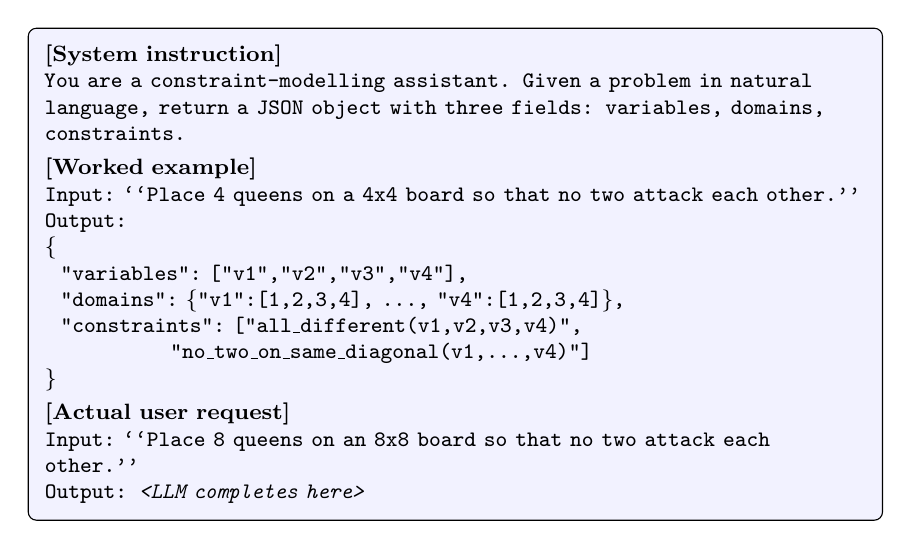
\begin{tikzpicture}[font=\footnotesize]
\node[draw, rounded corners=3pt, fill=blue!5, line width=0.4pt,
      inner sep=6pt, text width=0.86\linewidth, align=left] (p) {%
\textbf{[System instruction]}\\
\texttt{You are a constraint-modelling assistant. Given a problem in natural}\\
\texttt{language, return a JSON object with three fields: variables, domains,}\\
\texttt{constraints.}\\[3pt]
\textbf{[Worked example]}\\
\texttt{Input:\ ``Place 4 queens on a 4x4 board so that no two attack each other.''}\\
\texttt{Output:}\\
\texttt{\{}\\
\texttt{\ \ "variables":\ ["v1","v2","v3","v4"],}\\
\texttt{\ \ "domains":\ \{"v1":[1,2,3,4],\ ...,\ "v4":[1,2,3,4]\},}\\
\texttt{\ \ "constraints":\ ["all\_different(v1,v2,v3,v4)",}\\
\texttt{\ \ \ \ \ \ \ \ \ \ \ \ \ \ \ \ "no\_two\_on\_same\_diagonal(v1,...,v4)"]}\\
\texttt{\}}\\[3pt]
\textbf{[Actual user request]}\\
\texttt{Input:\ ``Place 8 queens on an 8x8 board so that no two attack each other.''}\\
\texttt{Output: \textit{<LLM completes here>}}
};
\end{tikzpicture}
\caption{Anatomy of the formaliser prompt. A system instruction states the task, a worked example shows the expected input--output shape (here for 4-Queens), and the actual request follows. The LLM completes the empty Output field below the request.}
\label{fig:prompt-anatomy}
\end{figure}

The model axis $m$ selects the specific LLM. Models differ in how many parameters they contain, in the data on which they were trained, and in whether they have been fine-tuned to produce explicit reasoning traces. These differences affect both per-call accuracy and per-call response time.

The agentic-design axis $\alpha$ specifies how many agents the system contains and how the output of one agent is passed to the next. The simplest agentic design uses a single agent for the whole task. A deeper agentic design splits the task into sub-tasks and assigns each sub-task to a dedicated agent. The four agentic designs studied in this work are described in Section~\ref{sec:method:pda}.

\subsection{Self-correcting systems}\label{sec:bg:refine}
A self-correcting system contains a loop that reads its own failure signals and tries again~\cite{R4}. A \emph{failure signal} can be a compilation error from the Java compiler, a runtime exception from the solver, or a complaint from an internal LLM verifier. When a failure signal appears, the system re-invokes the LLM with the failure trace attached as additional context, and the LLM produces a new attempt. The new attempt is submitted to the solver again. The loop terminates when an attempt succeeds, or when a fixed retry budget is exhausted. This mechanism provides the operational answer to \rqthree{}: within its retry budget, the system recovers from typical errors without human intervention.

\subsection{Neuro-symbolic perspective}\label{sec:bg:neurosymbolic}
The system studied here is an instance of a wider class called \emph{neuro-symbolic}~\cite{R7}. A neuro-symbolic system pairs a \emph{neural} component that reasons probabilistically over natural language (here the LLM) with a \emph{symbolic} component that manipulates exact logical or mathematical objects (here the Choco solver). The specific task that the two components solve together is called the \emph{business logic} of the system: clinical decision rules in a medical-diagnosis chatbot, statutes and case law in a legal-advice assistant, the production of a Choco model from a natural-language CSP description in the present work.

The recurring engineering question across these systems is the same: how should the probabilistic part and the exact part be coupled so that the exact part remains the source of truth~\cite{R8}? The verifier-redundancy tax of Section~\ref{sec:discussion:tax} is one partial answer for the case of CSP solving.


\subsection{Related work on multi-agent LLM systems}\label{sec:bg:related}
Several frameworks split a single user request across multiple LLM agents that exchange messages. AutoGen~\cite{R5} provides a generic conversational scaffold. MetaGPT~\cite{R6} and similar role-specialisation frameworks (ChatDev and related systems) simulate a software-engineering team with explicit role specialisation and report measurable gains over single-agent baselines on tasks such as code writing, design, and debate.

One property of those tasks deserves attention. None of them includes an automatic, exact external checker that decides correctness without ambiguity~\cite{R8}. The present study evaluates the same multi-agent idea on a task that \emph{does} include such a checker (the Choco solver). The contrast between the two settings is the heart of Section~\ref{sec:discussion}.

% =============================================================
\section{Materials and Methods}\label{sec:method}

\subsection{The enumeration of design combinations}\label{sec:method:config}
The configuration space $\mathcal{C} = \Pi \times M \times A$ defined in Section~\ref{sec:intro:axes} was enumerated cell by cell. For each configuration $c \in \mathcal{C}$, the system was run on the same benchmark suite (the set of problems), and the same metrics were recorded. The cells were then compared on equal footing. The cell with the highest success rate provides the surface-level answer to \rqtwo{}. The shape of the response surface along each axis identifies which design choice drives that answer. The agentic-design axis is studied in particular depth in Sections~\ref{sec:method:pda} and~\ref{sec:results:delegation}.

\subsection{The agentic-design axis: Progressive Delegation Ablation}\label{sec:method:pda}

\subsubsection{The five behaviours}\label{sec:method:pda:behaviours}
Converting a natural-language CSP description into a verified solution requires five distinct behaviours. Every configuration on the ladder performs all five behaviours. What changes across configurations is the way the five behaviours are distributed across one or more agents.

\begin{itemize}[leftmargin=1.4em,topsep=2pt,itemsep=1pt]
  \item \textbf{Formalisation}: read the natural-language description and extract the variables, their domains, and the constraints.
  \item \textbf{Modelling}: generate Java code that expresses the formalisation against the Choco API.
  \item \textbf{Validation}: inspect the generated model before the solver is invoked, and flag any obvious mismatch with the original problem statement.
  \item \textbf{Refinement}: read the failure message returned by the compiler, the validator, or the solver, and produce a corrected model.
  \item \textbf{Explanation}: produce a textual description of the returned solution, expressed using the variables of the original problem.
\end{itemize}

\subsubsection{The four-rung ladder}\label{sec:method:pda:ladder}
The PDA defines four agentic designs, denoted L0, L1, L2, and L3. The four designs are built by successive specialisation. L0 contains a single agent (the \emph{monolith}) that performs all five behaviours. At each higher rung, one behaviour is detached from the monolith and given to a new dedicated agent. The agent-to-behaviour assignment is summarised in Table~\ref{tab:ladder} and illustrated in Figure~\ref{fig:ladder}.

\begin{table}[H]
\centering
\caption{The four-rung delegation ladder. F = Formalisation, M = Modelling, V = Validation, R = Refinement, E = Explanation.}
\label{tab:ladder}
\small
\begin{tabular}{lcccccc}
\toprule
\textbf{Level} & \textbf{Agents} & \textbf{F} & \textbf{M} & \textbf{V} & \textbf{R} & \textbf{E} \\
\midrule
L0 (Monolith)         & 1 & Monolith   & Monolith & Monolith  & Monolith & Monolith \\
L1 (Refiner split)    & 2 & Monolith   & Monolith & Monolith  & Refiner  & Monolith \\
L2 (Validator split)  & 3 & Monolith   & Monolith & Validator & Refiner  & Monolith \\
L3 (Formaliser split) & 4 & Formaliser & Modeller & Validator & Refiner  & Modeller \\
\bottomrule
\end{tabular}
\end{table}

\begin{figure}[H]
\centering
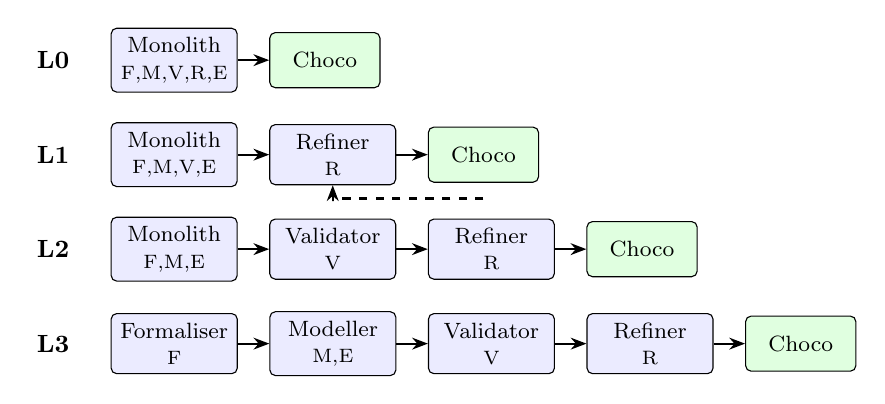
\begin{tikzpicture}[
  font=\footnotesize,
  node distance=4mm and 4mm,
  agent/.style={rectangle, draw, rounded corners=2pt, minimum height=7mm, minimum width=16mm, align=center, fill=blue!8},
  solver/.style={rectangle, draw, rounded corners=2pt, minimum height=7mm, minimum width=14mm, align=center, fill=green!12},
  level/.style={font=\bfseries\small},
  arr/.style={-{Stealth[length=2mm]}, thick},
]
\node[level] (lvl0) at (0,3.6) {L0};
\node[agent, right=of lvl0] (m0) {Monolith\\\scriptsize F,M,V,R,E};
\node[solver, right=of m0] (s0) {Choco};
\draw[arr] (m0) -- (s0);

\node[level] (lvl1) at (0,2.4) {L1};
\node[agent, right=of lvl1] (m1) {Monolith\\\scriptsize F,M,V,E};
\node[agent, right=of m1] (r1) {Refiner\\\scriptsize R};
\node[solver, right=of r1] (s1) {Choco};
\draw[arr] (m1) -- (r1);
\draw[arr] (r1) -- (s1);
\draw[arr, dashed] (s1.south) ++(0,-2mm) -| ($(r1.south)+(0,-2mm)$) -- (r1.south);

\node[level] (lvl2) at (0,1.2) {L2};
\node[agent, right=of lvl2] (m2) {Monolith\\\scriptsize F,M,E};
\node[agent, right=of m2] (v2) {Validator\\\scriptsize V};
\node[agent, right=of v2] (r2) {Refiner\\\scriptsize R};
\node[solver, right=of r2] (s2) {Choco};
\draw[arr] (m2) -- (v2);
\draw[arr] (v2) -- (r2);
\draw[arr] (r2) -- (s2);

\node[level] (lvl3) at (0,0) {L3};
\node[agent, right=of lvl3] (f3) {Formaliser\\\scriptsize F};
\node[agent, right=of f3] (md3) {Modeller\\\scriptsize M,E};
\node[agent, right=of md3] (v3) {Validator\\\scriptsize V};
\node[agent, right=of v3] (r3) {Refiner\\\scriptsize R};
\node[solver, right=of r3] (s3) {Choco};
\draw[arr] (f3) -- (md3);
\draw[arr] (md3) -- (v3);
\draw[arr] (v3) -- (r3);
\draw[arr] (r3) -- (s3);
\end{tikzpicture}
\caption{The four agentic designs of the PDA. The same five behaviours (F, M, V, R, E) are performed at every level; only the distribution across agents changes. The Refiner is invoked whenever a downstream component (compiler, validator, or solver) returns a failure signal; the dashed feedback edge is shown only at L1 for compactness, and exists at every level.}
\label{fig:ladder}
\end{figure}

The hypothesis tested by the PDA is straightforward. Splitting the five behaviours across specialised agents is expected to reduce the amount of work each agent does. A smaller per-agent workload is, in turn, expected to raise per-agent reliability. The aggregate effect should be a higher end-to-end success rate at L3 than at L0, together with improvements on the cost-side metrics (wall time and refinement iterations). This hypothesis is the operational form of the assumption that underlies multi-agent frameworks such as AutoGen~\cite{R5} and MetaGPT~\cite{R6}.

\subsection{The prompting axis}\label{sec:method:prompt}
Each agent on the ladder was given a prompting technique chosen for the behaviour the agent performs. The monolith uses few-shot prompting~\cite{R3} with two worked examples, because few-shot prompting is the most general technique and the monolith performs the broadest set of behaviours. The refiner uses a Reflexion-style prompt~\cite{R4}, because the refiner must read a previous failure and adapt its output, and Reflexion is the prompting family designed precisely for that purpose. The validator uses adversarial Chain-of-Thought prompting~\cite{R3}, because the validator must look for defects, and adversarial Chain-of-Thought encourages the LLM to enumerate possible defects before stating a verdict. The formaliser uses structured output through a Pydantic schema, because the output of the formaliser is consumed directly by the next agent, and must therefore be parsable without ambiguity.

\subsection{The model axis}\label{sec:method:models}
Three LLMs were selected to cover deliberately different profiles. Qwen 2.5-Coder-32B was chosen because it is an open model fine-tuned on code, and therefore serves as a code-generation baseline. Claude Haiku 4.5 was chosen because it is a small commercial model with low response time and high single-call accuracy on short instructions. DeepSeek-R1-Distill-Llama-70B was chosen because it has been trained with explicit reasoning traces, which makes it possible to test whether reasoning-oriented training compensates for delegation depth. All three models were accessed through OpenRouter, a network gateway that exposes models from many providers behind a single uniform interface. OpenRouter was chosen because identical request semantics across providers remove one source of measurement variability.

\subsection{The self-correction loop}\label{sec:method:refine}
The self-correction loop is present at every level of the PDA. The loop is triggered by three failure conditions. The first condition is a compilation error reported by Maven on the generated Java code. The second condition is a runtime exception thrown by Choco during search. The third condition is the absence of a valid solution after the solver has finished. When any of the three conditions occurs, the refining behaviour is invoked with the corresponding failure trace as additional context. The refiner produces a new model, and the new model is re-submitted to Choco. The loop terminates when Choco accepts the model, or when the retry counter reaches the constant \texttt{MAX\_REFINEMENT\_ITERATIONS}, set to three for every experiment. The loop is the operational answer to \rqthree{}; its convergence behaviour is reported in Section~\ref{sec:results:cost}.

\subsection{Enumeration procedure}\label{sec:method:enum}
The configurations were enumerated by a triple-nested loop, shown below. The outer loop iterates over the four delegation levels. The middle loop iterates over the three LLMs. The inner loop iterates over the ten benchmark problems. The total number of runs is therefore $|A| \times |M| \times |B| = 4 \times 3 \times 10 = 120$.

\begin{lstlisting}[language=Python]
for level in {L0, L1, L2, L3}:
    workflow = build_workflow(level)
    for model in {Qwen, Haiku, DeepSeek}:
        for problem in benchmarks:
            run = workflow.solve(problem, model)
            record_metrics(run)
\end{lstlisting}

\subsection{Benchmark suite}\label{sec:method:bench}
Ten CSP instances were drawn from CSPLib~\cite{R2}, the standard benchmark library used in the constraint-programming community. The instances include 4-Queens and 8-Queens (CSPLib problem 054), Magic Square (problem 019), SEND + MORE = MONEY (problem 023), Graph Colouring (problem 004), Latin Square (problem 003), and Sudoku (problem 028). The remaining instances cover a scheduling problem, a knapsack problem, and a cryptarithmetic variant. The suite is partitioned into three difficulty tiers (easy, medium, hard). The hard tier contains four instances and is the tier where the effects along the agentic-design axis appear (Section~\ref{sec:results:hard}). Reusing CSPLib problems rather than designing new ones was chosen because CSPLib makes the present results directly comparable with prior constraint-programming work.

\subsection{Metrics}\label{sec:method:metrics}
Each metric is tied to one or more research questions. The \emph{success rate} (the fraction of problems for which Choco returned a valid solution) addresses \rqone{} and \rqtwo{}. The \emph{first-shot success rate} (the fraction of problems solved at iteration zero, before any refinement was needed) and the \emph{mean number of refinement iterations} address \rqthree{}. The \emph{compilation-failure rate} (the fraction of runs in which the generated Java did not compile) addresses \rqone{}. The \emph{wall time per problem} and the Choco \emph{solver statistics} (nodes explored, backtracks, propagations) inform the cost analysis of \rqtwo{}. A regex-based \emph{explanation-faithfulness score}, which counts how many of the solver's variable names also appear in the textual explanation produced by the LLM, was also recorded. The score's limitations are reported in Section~\ref{sec:discussion:limits}.

\subsection{Tools and reproducibility}\label{sec:method:tools}
The symbolic component is Choco Solver~\cite{R1}, a Java constraint-programming library. Generated Java models were compiled by Apache Maven and executed in a dedicated subprocess. The agent graphs were implemented in LangGraph, a Python library for building state-machine-style LLM workflows. LangGraph was chosen because the per-level workflow can be expressed as a graph in which each node is one LLM call and each edge is a conditional transition. LLM calls were routed through OpenRouter, as explained in Section~\ref{sec:method:models}. LangSmith was used to trace and store every LLM call. Choco is deterministic with respect to its Java input: identical generated source produces identical output and identical search statistics on every run. The only non-deterministic part of every measurement is therefore the LLM call itself.

% =============================================================
\section{Results}\label{sec:results}

The results are reported along the three design axes. The success rate per cell is the headline metric. The cost-side metrics (compilation failures, refinement iterations, wall time) are reported separately. All values are computed over the ten-problem suite of Section~\ref{sec:method:bench}.

\subsection{The configuration grid}\label{sec:results:grid}
The success rate of each cell of the (level, model) grid is reported in Table~\ref{tab:grid}. The L0 row is uniformly at $100\%$, independent of the LLM. The L3 row ranges between $50\%$ and $90\%$ depending on the LLM. The grid identifies the cells at $\alpha = $ L0, for any model, as the highest-performing configurations under the tested conditions.

\begin{table}[H]
\centering
\caption{Success rate per configuration cell. Rows: delegation levels. Columns: LLMs. Values are percentages over the ten-problem suite.}
\label{tab:grid}
\small
\begin{tabular}{lccc|c}
\toprule
 & \textbf{Qwen 2.5-Coder-32B} & \textbf{Haiku 4.5} & \textbf{DeepSeek-R1 70B} & \textbf{Mean} \\
\midrule
L0 & 100 & 100 & 100 & 100.0 \\
L1 & 100 & 100 & 80  & 93.3 \\
L2 & 90  & 50  & 100 & 80.0 \\
L3 & 90  & 60  & 50  & 66.7 \\
\bottomrule
\end{tabular}
\end{table}

\subsection{Variation along the delegation axis}\label{sec:results:delegation}
The strongest pattern in the grid lies along the agentic-design axis $\alpha$. Figure~\ref{fig:success-curve} reports the success rate of each LLM at each level, together with the mean across the three LLMs. The mean decreases at every step: $100.0\% \to 93.3\% \to 80.0\% \to 66.7\%$. The total loss between L0 and L3 is $33.3$ percentage points. Two of the three LLMs, Qwen and Haiku, also decrease individually between L1 and L3. DeepSeek alternates across levels but ends at $50\%$ at L3, half of its L0 value.

\begin{figure}[H]
\centering
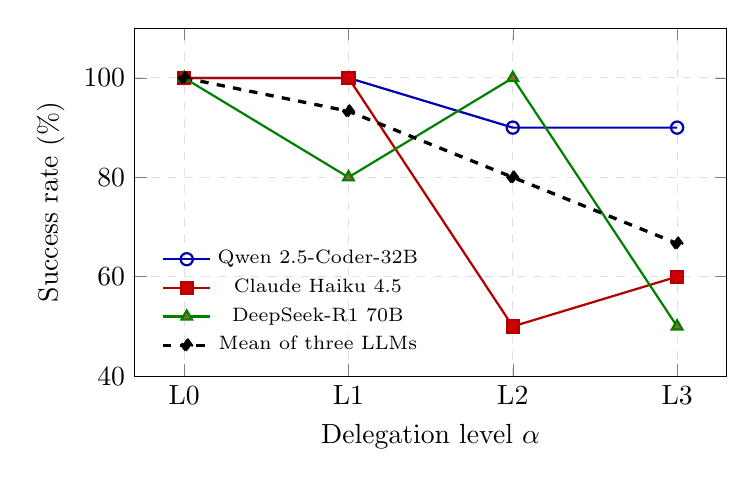
\begin{tikzpicture}
\begin{axis}[
  width=0.75\linewidth, height=6cm,
  xlabel={Delegation level $\alpha$}, ylabel={Success rate (\%)},
  xtick={0,1,2,3}, xticklabels={L0,L1,L2,L3},
  ymin=40, ymax=110, ytick={40,60,80,100},
  legend pos=south west, legend style={font=\scriptsize, draw=none, fill=none},
  grid=both, grid style={dashed,gray!25},
  every axis plot/.append style={thick, mark options={scale=1.1}},
]
\addplot+[mark=o, color=blue!70!black]
  coordinates {(0,100) (1,100) (2,90) (3,90)};
\addlegendentry{Qwen 2.5-Coder-32B}
\addplot+[mark=square*, color=red!70!black]
  coordinates {(0,100) (1,100) (2,50) (3,60)};
\addlegendentry{Claude Haiku 4.5}
\addplot+[mark=triangle*, color=green!50!black]
  coordinates {(0,100) (1,80) (2,100) (3,50)};
\addlegendentry{DeepSeek-R1 70B}
\addplot+[mark=diamond*, dashed, color=black, very thick]
  coordinates {(0,100) (1,93.3) (2,80) (3,66.7)};
\addlegendentry{Mean of three LLMs}
\end{axis}
\end{tikzpicture}
\caption{Success rate against delegation level $\alpha$. The mean across the three LLMs decreases monotonically as the number of agents grows.}
\label{fig:success-curve}
\end{figure}

\subsection{Variation along the model axis}\label{sec:results:models}
The three LLMs exhibit three distinct response profiles along the delegation axis. Qwen 2.5-Coder-32B is the most stable: it loses ten percentage points between L1 and L2 and remains at $90\%$ at L3. Claude Haiku 4.5 ties for the strongest LLM at L0 and L1 ($100\%$), but falls to $50\%$ at L2. DeepSeek-R1 70B is the only LLM whose L2 value ($100\%$) exceeds its L1 value ($80\%$); it then drops to $50\%$ at L3. The ranking of the three LLMs is therefore not preserved across levels. Performance at L0 does not predict performance at L3.

\subsection{Hard-tier breakdown}\label{sec:results:hard}
The easy and medium tiers were solved at or near $100\%$ across every cell. The entire effect of the delegation axis lives in the four hard-tier problems. Figure~\ref{fig:hard} reports the count of hard-tier problems solved at each level for each LLM (out of four per LLM). The total across the three LLMs falls from $12/12$ at L0 to $5/12$ at L3. The four hard problems that fail at the deeper levels are Sudoku, SEND + MORE = MONEY, the scheduling instance, and the knapsack instance.

\begin{figure}[H]
\centering
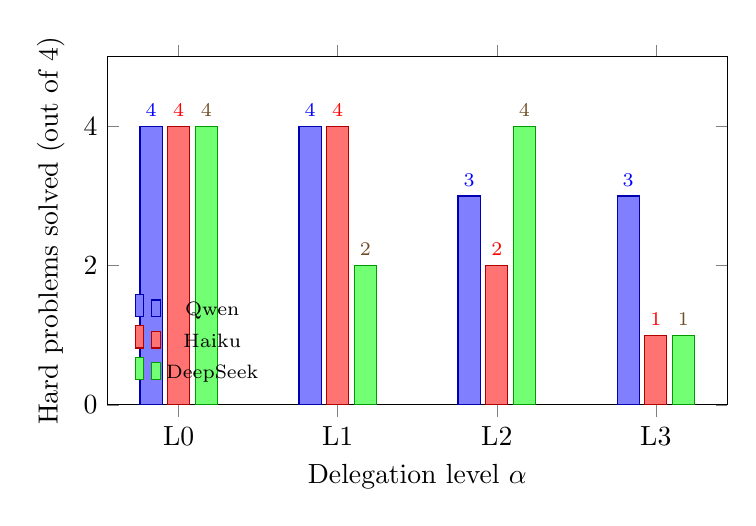
\begin{tikzpicture}
\begin{axis}[
  width=0.78\linewidth, height=6cm,
  ybar, bar width=8pt,
  ymin=0, ymax=5,
  xlabel={Delegation level $\alpha$}, ylabel={Hard problems solved (out of 4)},
  symbolic x coords={L0,L1,L2,L3},
  xtick=data,
  legend pos=south west, legend style={font=\scriptsize, draw=none, fill=none},
  enlarge x limits=0.15,
  nodes near coords, nodes near coords style={font=\scriptsize},
]
\addplot+[fill=blue!50, draw=blue!70!black]
  coordinates {(L0,4) (L1,4) (L2,3) (L3,3)};
\addlegendentry{Qwen}
\addplot+[fill=red!55, draw=red!70!black]
  coordinates {(L0,4) (L1,4) (L2,2) (L3,1)};
\addlegendentry{Haiku}
\addplot+[fill=green!55, draw=green!60!black]
  coordinates {(L0,4) (L1,2) (L2,4) (L3,1)};
\addlegendentry{DeepSeek}
\end{axis}
\end{tikzpicture}
\caption{Hard-tier success per LLM and per level (out of four hard problems per LLM). The total across the three LLMs falls from $12/12$ at L0 to $5/12$ at L3.}
\label{fig:hard}
\end{figure}

\subsection{The cost dimension}\label{sec:results:cost}
Three cost-side metrics deepen the picture. First, the compilation-failure rate rises from $0\%$ at L0 to approximately $27\%$ at L3. Second, the mean number of refinement iterations approximately triples between L0 and L3. Third, the mean wall time per problem grows from $47$ seconds at L0 to $788$ seconds at L3, a factor of sixteen.

The L3 wall-time mean is, however, distorted by a single outlier. One DeepSeek run on SEND + MORE = MONEY reported an elapsed time of $21\,318$ seconds. Inspection of the trace showed that the elapsed time was not produced by model reasoning, but by a stalled HTTP request to the provider, which eventually returned a timeout error. The corresponding run produced no Java code and triggered no refinement iteration. Removing this single run lowers the L3 mean wall time appreciably. The qualitative ordering of the four levels (L0 $<$ L1 $<$ L2 $<$ L3 in wall time) is preserved with or without the outlier.

The compilation-failure trajectory of Claude Haiku 4.5 is reported separately in Figure~\ref{fig:haiku-cf}. Its non-monotonic shape ($0\%$ at L0, $0\%$ at L1, $50\%$ at L2, $30\%$ at L3) is the strongest evidence for mechanism M3 of Section~\ref{sec:discussion:mechanisms}.

\begin{figure}[H]
\centering
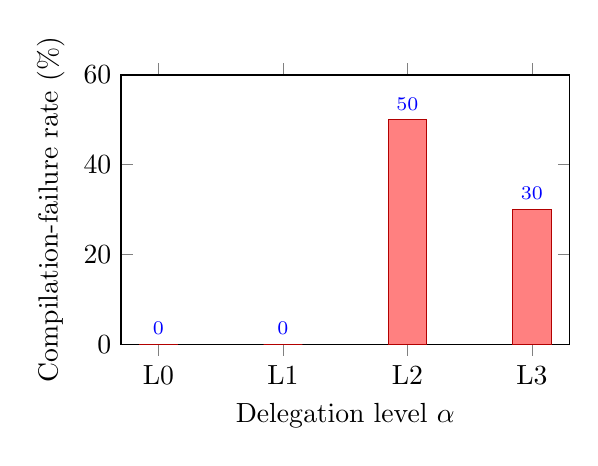
\begin{tikzpicture}
\begin{axis}[
  width=0.6\linewidth, height=5cm,
  ybar, bar width=14pt,
  ymin=0, ymax=60,
  xlabel={Delegation level $\alpha$}, ylabel={Compilation-failure rate (\%)},
  symbolic x coords={L0,L1,L2,L3},
  xtick=data,
  nodes near coords, nodes near coords style={font=\scriptsize},
]
\addplot+[fill=red!50, draw=red!70!black]
  coordinates {(L0,0) (L1,0) (L2,50) (L3,30)};
\end{axis}
\end{tikzpicture}
\caption{Claude Haiku 4.5: compilation-failure rate per delegation level. The jump at L2 coincides with the introduction of the validator into the system.}
\label{fig:haiku-cf}
\end{figure}

\subsection{Verdict on the pre-registered predictions}\label{sec:results:verdict}
Four directional predictions were registered before the measurements were taken. The predictions and the observed outcomes are reported in Table~\ref{tab:verdict}. All four predictions were refuted by the data.

\begin{table}[H]
\centering
\caption{Pre-registered predictions and observed outcomes.}
\label{tab:verdict}
\small
\begin{tabular}{lll}
\toprule
\textbf{Rung} & \textbf{Prediction} & \textbf{Observation} \\
\midrule
L1 vs.\ L0 & Mean success up                  & Mean success down (100 $\rightarrow$ 93.3) \\
L2 vs.\ L1 & Mean success up; iterations down & Both refuted \\
L3 vs.\ L2 & Mean success up on hard tier     & Hard tier 9/12 $\rightarrow$ 5/12 \\
\bottomrule
\end{tabular}
\end{table}

% =============================================================
\section{Discussion}\label{sec:discussion}

\subsection{Identifying the best configuration}\label{sec:discussion:best}
On the benchmark suite tested, the configurations with the highest success rate are those at the shallowest delegation level. The L0 row of Table~\ref{tab:grid} is uniformly at $100\%$, whatever the LLM. The surface-level answer to \rqtwo{} is therefore the monolithic configuration. The remaining question is why the deeper configurations, which the multi-agent-LLM literature treats as beneficial, fail to improve upon L0 on the present task. The rest of Section~\ref{sec:discussion} addresses that question through five mechanisms (Section~\ref{sec:discussion:mechanisms}) and one unifying principle (Section~\ref{sec:discussion:tax}).

\subsection{Five mechanisms behind the decline}\label{sec:discussion:mechanisms}
Five mechanisms are proposed. Each mechanism is tied to a specific datum reported in Section~\ref{sec:results}.

\textbf{M1 -- Errors stack up across stages.} A system composed of $k$ sequential stages, each correct with probability $p$, has joint correctness bounded above by $p^k$. With $p = 0.95$ and $k = 4$, the bound is approximately $0.81$. M1 alone accounts for a $19$ percentage-point gap between L0 and L3. The observed mean gap is $33.3$ percentage points. The remaining $14$ points must therefore come from other mechanisms.

\textbf{M2 -- Redundancy with the external checker.} Choco is a deterministic and exact checker: either the generated model compiles and yields a valid solution, or it does not. Placing a probabilistic LLM critic above an exact checker adds noise to the decision without adding information. The expected contribution of the critic is at best zero, and becomes negative whenever the critic flags correct code as faulty.

\textbf{M3 -- The critic introduces its own bugs.} A prompt that asks the validator to find defects rarely returns an empty answer. The validator therefore tends to flag correct code. The refiner, which is instructed to trust the validator, then modifies the flagged code. The modification can introduce errors that were not present in the original model. The strongest evidence is the compilation-failure trajectory of Claude Haiku 4.5 in Figure~\ref{fig:haiku-cf}. Haiku produced no compilation failures at L0 or L1, but produced compilation failures on half of its runs at L2 once the validator was added. Half of the L2 compilation failures were therefore introduced by the loop itself rather than by the original generator.

\textbf{M4 -- The retry budget is blind to the cost of one retry.} The retry budget was fixed to three at every level. At L0, one retry corresponds to one LLM call. At L3, one retry corresponds to approximately four LLM calls, because the entire agent chain is re-traversed on each attempt. The same nominal budget therefore consumes very different amounts of compute. A budget calibrated for L0 is too small to recover the genuinely hard cases at L3, and disproportionately expensive on cases that have already failed.

\textbf{M5 -- LLMs react differently to delegation.} The three LLMs exhibit three different decline profiles along $\alpha$ (Section~\ref{sec:results:models}). Haiku leads at L0 and L1, then collapses at L2. DeepSeek alternates. Qwen remains the most stable. No single ranking of the three LLMs is preserved across the four levels. The performance of an LLM on the monolithic configuration is therefore not a reliable predictor of its performance under deeper delegation.

\subsection{The verifier-redundancy tax}\label{sec:discussion:tax}
The five mechanisms can be unified under one principle. Multi-agent decomposition is beneficial when it \emph{substitutes} for a missing external checker, as in essay writing, code review without execution, or open-ended dialogue. Multi-agent decomposition is harmful when it \emph{competes} with an external checker that is already exact and deterministic, as in CSP solving against a complete solver~\cite{R8}. On the benchmark suite tested here, the harm amounts to a loss of approximately $7$ to $13$ percentage points of mean success rate per added agent. This work names that loss the \emph{verifier-redundancy tax}, a CSP-specific instance of the broader LLM-Modulo principle of Kambhampati et al.~\cite{R8}. The principle is the contribution restated from Section~\ref{sec:intro:contrib}.

\subsection{Relation to prior literature}\label{sec:discussion:relation}
The results presented here do not contradict prior multi-agent work. AutoGen~\cite{R5}, MetaGPT~\cite{R6}, and ChatDev evaluate decomposition on tasks for which no automatic external checker exists. On those tasks, decomposition reports gains over single-agent baselines. The present study suggests that the gains do not transfer to tasks for which an external checker already exists. The present work supplies the missing controlled comparison: the same five behaviours, the same benchmark suite, the same exact checker, varied only along the agentic depth. The contribution of the present work is therefore to restrict, not to refute, the scope of the prior claims.

\subsection{Limitations}\label{sec:discussion:limits}
Five limitations should be made explicit before the present results are generalised.

First, the hard tier of the benchmark contains four problems per LLM, for a total of twelve cells per level. The mean trend is monotonic, but the per-cell differences fall within one standard error. A larger benchmark would be required to estimate the per-level effect size more precisely.

Second, the Choco statistics parser produced suspiciously constant values for nodes, backtracks, and propagations across instances of very different sizes. Fine-grained comparisons of search effort across configurations were therefore not possible on the current logs.

Third, the regex-based explanation-faithfulness score returned zero on every run, because the underlying solution dictionary remained empty during logging. The score is therefore structurally undefined for the runs collected here. A different scoring protocol (for example, an LLM-as-judge protocol) would be required to evaluate explanation quality.

Fourth, per-call token counts were not persisted. The cost-decoupling argument associated with L3 cannot be quantified on the current data.

Fifth, only sequential decomposition was tested. The verifier-redundancy tax was observed for a chain topology. Whether the principle generalises to alternative topologies (debate, voting, tree-structured agentic designs) is left for future work.

% =============================================================
\section{Conclusion}\label{sec:conclusion}

\subsection{Summary}\label{sec:conclusion:summary}
This work introduces an enumeration of all design combinations for an LLM-driven CSP-solving system. Three design choices were varied jointly: the prompting technique $\pi$, the LLM $m$, and the agentic design $\alpha$. The agentic-design axis was then studied in depth through the Progressive Delegation Ablation (PDA), which compares four system depths from a single all-in-one agent (L0) to a chain of four specialised agents (L3). On the ten-problem benchmark suite tested, the mean success rate falls monotonically from $100\%$ at L0 to $66.7\%$ at L3, and the four hard-tier problems account for the entire decline. Five mechanisms (M1 to M5) are proposed to explain the decline. The five mechanisms are unified under a single principle, the \emph{verifier-redundancy tax}: multi-agent decomposition tends to compete with, rather than complement, an external checker that is already exact. The contribution of the present work is therefore both empirical (a refutation of the pre-registered hypothesis under the tested conditions) and methodological (a principle that delimits when multi-agent decomposition is expected to help).

\subsection{Future work}\label{sec:conclusion:future}
Six directions follow directly from the limitations of Section~\ref{sec:discussion:limits}. First, the delegation order could be reversed (formaliser first, then validator, then refiner) to test whether a different error profile emerges. Second, the validator could be allowed to abstain rather than be required to produce a critique, which would directly test mechanism M3. Third, the retry budget could be made level-aware, scaling with the per-iteration LLM-call count. Fourth, the Choco statistics parser should be corrected before any further claim on search effort is drawn. Fifth, the hard tier should be expanded to at least twelve problems per LLM to obtain adequate statistical power. Sixth, non-sequential agentic designs (debate, voting, tree-structured) should be evaluated against the verifier-redundancy tax to test the generality of the principle.

% =============================================================

\begin{thebibliography}{99}

\bibitem{R1} C. Prud'homme and J.-G. Fages, ``Choco-solver: A Java library for constraint programming,'' \emph{Journal of Open Source Software}, vol. 7, no. 78, p. 4708, 2022. doi: 10.21105/joss.04708.

\bibitem{R2} I. P. Gent and T. Walsh, ``CSPLib: A benchmark library for constraints,'' in \emph{Principles and Practice of Constraint Programming (CP'99)}, Lecture Notes in Computer Science, vol. 1713. Berlin, Heidelberg: Springer, 1999, pp. 480--481. [Online]. Available: \url{https://www.csplib.org}

\bibitem{R3} J. Wei, X. Wang, D. Schuurmans, M. Bosma, B. Ichter, F. Xia, E. Chi, Q. Le, and D. Zhou, ``Chain-of-thought prompting elicits reasoning in large language models,'' in \emph{Advances in Neural Information Processing Systems (NeurIPS)}, vol. 35, 2022. arXiv:2201.11903.

\bibitem{R4} N. Shinn, F. Cassano, A. Gopinath, K. Narasimhan, and S. Yao, ``Reflexion: Language agents with verbal reinforcement learning,'' in \emph{Advances in Neural Information Processing Systems (NeurIPS)}, vol. 36, 2023. arXiv:2303.11366.

\bibitem{R5} Q. Wu, G. Bansal, J. Zhang, Y. Wu, B. Li, E. Zhu, L. Jiang, X. Zhang, S. Zhang, J. Liu, A. H. Awadallah, R. W. White, D. Burger, and C. Wang, ``AutoGen: Enabling next-generation large language model applications via multi-agent conversation,'' arXiv preprint arXiv:2308.08155, 2023.

\bibitem{R6} S. Hong, X. Zheng, J. Chen, Y. Cheng, C. Zhang, Z. Wang, S. K. S. Yau, Z. Lin, L. Zhou, C. Ran, L. Xiao, and C. Wu, ``MetaGPT: Meta programming for a multi-agent collaborative framework,'' in \emph{International Conference on Learning Representations (ICLR)}, 2024. arXiv:2308.00352.

\bibitem{R7} Z. Wan, C.-K. Liu, H. Yang, C. Li, H. You, Y. Fu, C. Wan, T. Krishna, Y. Lin, and A. Raychowdhury, ``Towards cognitive AI systems: A survey and prospective on neuro-symbolic AI,'' arXiv preprint arXiv:2401.01040, 2024.

\bibitem{R8} S. Kambhampati, K. Valmeekam, L. Guan, M. Verma, K. Stechly, S. Bhambri, L. Saldyt, and A. Murthy, ``LLMs can't plan, but can help planning in LLM-Modulo frameworks,'' in \emph{Proceedings of the 41st International Conference on Machine Learning (ICML)}, 2024. arXiv:2402.01817.

\bibitem{R9} F. R{\'e}gin, E. De Maria, and A. Bonlarron, ``Combining constraint programming reasoning with large language model predictions,'' in \emph{Proceedings of the 30th International Conference on Principles and Practice of Constraint Programming (CP 2024)}, LIPIcs, vol. 307, art. 25, 2024. doi: 10.4230/LIPIcs.CP.2024.25.

\bibitem{R10} S. Szeider, ``CP-Agent: Agentic constraint programming,'' arXiv preprint arXiv:2508.07468, 2025.

\end{thebibliography}

\end{document}
